\documentclass[11pt]{refart}
\usepackage[utf8]{inputenc}
\usepackage[english]{babel}

\usepackage{subfigure}
\usepackage{graphicx}
\usepackage{tikz}
\usetikzlibrary{shadows}
\usepackage{xspace}
\usepackage{moreverb} % control tabs in verbatim
\usepackage{tcolorbox}
\usepackage{xcolor}
\usepackage[bottom]{footmisc}
\usepackage[hidelinks]{hyperref}

\hypersetup{
    colorlinks,
    linkcolor={red!60!black},
    citecolor={blue!60!black},
    urlcolor={blue!80!black}
}
\newcommand{\button}[1]%
{   
	\begin{tikzpicture}[baseline=(tempname.base)]
        \node[draw=gray, fill=yellow!5, rounded corners=.2ex, inner xsep=.5em, minimum width=1.5em, minimum height=1.5em] (tempname) {#1};
    \end{tikzpicture}
}
\newcommand{\marginicon}[2][]{\marginlabel{\raisebox{-.1\height}{\includegraphics[#1]{#2}}}}

\makeatletter
\newcommand{\verbatimfont}[1]{\renewcommand{\verbatim@font}{\ttfamily#1}}
\makeatother

\newtcolorbox{screenBox}[1][]
{
  %boxrule=0pt,
  colback  = white!95!gray,
  #1,
}
\newenvironment{fullfigure}[1][ht]
{%
\begin{figure}[#1]%
  	\hspace*{-\leftmarginwidth}%
  	\begin{minipage}{\fullwidth}%
}%
{%
	\end{minipage}%
\end{figure}%
}
\newenvironment{screenshots}[1][ht]
{
\begin{figure}[#1]
\begin{screenBox}
\centering
}
{\end{screenBox}\end{figure}}
\newcommand{\screenshot}[3]{%
	\subfigure[#2]{%
		\includegraphics[scale=.5]{#1}%
		\label{#3}%
	}
}
\newcommand{\singlescreenshot}[4][]{%
	\begin{figure}[ht]%
	\begin{screenBox}%
		\centering
  		\includegraphics[scale=.5,#1]{#2}%	
  		\caption{#3}%
  		\label{#4}%
  	\end{screenBox}
	\end{figure}%	
}
\newcommand{\fullscreenshot}[3]{%
	\begin{fullfigure}[ht]%
  		\includegraphics[scale=.5]{#1}%
  		\caption{#2}%
  		\label{#3}%
	\end{fullfigure}%	
}
 
\newcommand*{\marginparagraph}[1]{\marginlabel{\textbf{#1}}}
\newcommand*{\textAtt}[1]{\attention\underline{#1}}

\newcommand*{\socketsender}{SocketSenderGUI\xspace}
\newcommand*{\msg}{\texttt{message}\xspace}
\newcommand*{\sequence}{\texttt{sequence}\xspace}
\newcommand*{\newButton}{\button{New}\xspace}
\newcommand*{\saveButton}{\button{Save}\xspace}
\newcommand*{\saveAsButton}{\button{Save As}\xspace}
\newcommand*{\deleteButton}{\button{Delete}\xspace}
\newcommand*{\useMessageButton}{\button{Use this message}\xspace}
\newcommand*{\useSequenceButton}{\button{Use this sequence}\xspace}
\newcommand*{\useCustomMessageButton}{\button{Use this custom message}\xspace}
\newcommand*{\useCustomSequenceButton}{\button{Use this custom sequence}\xspace}

\title{PISA Server Graphical Interface\\The Manual}
\author{\copyright Andrei Dorman (AD250303)}
\date{\today}

\makeindex

\begin{document}

\maketitle
\vfill
\tableofcontents

\pagebreak

\null
\vfill
\section{Introduction}

This tool, \socketsender, is a simple message sender that \emph{simulates} messages an app can send to a web renderer.
This way, a developer working on the graphics for a customer can avoid actually using the larger app, maybe on a virtual machine, restarting it on every problem, re-playing the scenario that brings to a given screen again and again, modifying other server responses to simulate error messages, etc. 

\marginlabel{Messages and Sequences}
The principal block of data exchange is the \emph{message}. 
The message can be used to send all the info for a screen, or just for part of a page.
It can be in fact any interaction between the app and the renderer.
Sometimes the developer will want a sequence of screens to appear one after the other to simulate the ongoing of some simple process. 

For this purpose, this tool makes use of \emph{sequences} that are nothing else than lists of messages eventually separated by pauses.
For now, sequences can only be composed of two types of elements: messages of course, and a \emph{wait} function that takes a number of \emph{milliseconds} to wait between a step and the next.
A future development could introduce the use of function calls directly as parts of a sequence.

We will refer indifferently to a message or a sequence as an \emph{action}. 
We will say an action has been \emph{picked} when it is the one chosen to be sent to the renderer.

\pagebreak
\section{The window: the Message Picker}

\fullscreenshot{../screenshots/01_MainWindow.png}{The Main Window}{fig:mainWindow}

The user interface is quite simple.
A single window (\autoref{fig:mainWindow}) allows to manage the collection of messages and sequences and to pick an action from these collections to be sent to the renderer.

\subsection*{The left pane: choose what to send}
\label{sec:leftPane}

The left pane is composed of various \emph{lists} and a \emph{filter bar}.
The first column lists the saved messages.
The second columns, on top, lists the saved sequences.
When a sequence is selected, the bottom part of that columns lists the different \emph{steps} of that sequence.

Selecting an element in one of the lists \textAtt{does not} \emph{pick} it to be used.
It just shows its content in the editor (on the right pane, see next section).

\marginlabel{Pick a message}
Clicking the button under a list actually picks the selected element to be sent to the renderer. 
Notice that buttons are enable or disabled depending on which kind of element is selected.

\marginlabel{Current message}
The \emph{currently used action} has a colored background -- light blue -- different from the color of a selected item.
When an action is picked, it is saved as current action and automatically loaded on next startup.

\marginlabel{Filter}
The \emph{filter bar} allows to filter all the lists, removing all messages that do not fit the text.
It is case-insensitive and filters both messages and sequences.
For more details, see \ref{sec:filterBar}.

\subsection*{The right pane: the editor and manager}
\label{sec:rightPane}

The \emph{editor} is a minimal Json editor (coloring and folding). 
When an action is selected, its content appears in the editor, this way the developer can check it and modify it.

\attention Notice how as soon as the text has been modified, the button underneath changes from ``Use this message'' to ``Use this custom message''. 
This way, the developer is reminded he has modified and not saved the action. 
\marginlabel{Custom action}
A \emph{custom message} or \emph{custom sequence} can be picked and is saved for a next session like any other current message.

The buttons under the editor are self-explanatory.
For a more detailed overview of the processes of saving, creating or deleting, see respectively \ref{sec:save}, \ref{sec:new} and \ref{sec:delete}.

\marginlabel{Status bar}
In the mini-status bar on the bottom right, the progress bar shows that the server is \emph{running}: the picked action is sent to the renderer whenever this latter connects to the message server (basically, on every refresh of the page, since we are talking about a browser renderer).
The last button on the right opens (and closes) the \emph{config file} in the editor. 
Its is a Json string itself (see \autoref{sec:configuration} for details).


\section{Configuration}
\label{sec:configuration}

\marginicon[scale=0.5]{../icons/1481130257_Working_Tools_2}
To open the configuration file, click that button in the the bottom right. 
It will load the file in a Json editor. 
To close, click the same button again:
it will \textAtt{save automatically} the configuration on close.

\marginlabel{On first open}
A warning message might appear if the configuration is not set yet.

Setting up the configuration means choosing a destination \emph{HTML5 renderer project} and some paths to where to save actions: one for messages, one for sequences, and one for the current action, whatever type it is.

\begin{screenBox}[colbacktitle=white, coltitle=black, title=The configuration file]
\footnotesize
\begin{verbatimtab}[3]
{
	"Customer": "CrAsti",
	"Customers" : {
		"SuperStoreApp": {
			"HtmlWebPath" : "C:\\HTMLProjects\\Html5_SuperStore",
			"MessagesPath" : "actions\\messages",
			"SequencesPath" : "actions\\sequences",
			"CurrentActionPath" : "actions\\current"
		},
		"Default": {
			"HtmlWebPath" : "",
			"MessagesPath" : "actions\\messages",
			"SequencesPath" : "actions\\sequences",
			"CurrentActionPath" : "actions\\current"
		}
	}
}
\end{verbatimtab}
\end{screenBox}

In order to be able to work with various projects, \socketsender can ``remember'' a \emph{project} per customer.
Each project in nothing else than a name and a configuration.
This way, each customer can have its own personalized sets of actions.

One can just change the value of the \verb+Customer+ parameter to one of the \verb+Customers'+ name in order to switch from one project to another.

All paths can be relative or absolute.
Note that the backslashes need to be \textAtt{escaped} as the strings are not formatted by the deserializer.

\section{Manage messages and sequences}

\subsection{Filter}
\label{sec:filterBar}

%\screenshot{../screenshots/12_Filter_NotInSubsequence.png}{Filter messages and sequences}{fig:filteredNotInside}

The filter is instantaneous: all lists are filtered on every keystroke.
The option \emph{in details} lets you choose to keep the sequences which contain a message that corresponds to the filter even if the name of the sequence itself does not.

\begin{fullfigure}
  	\subfigure[Keep sequences that contain a filtered message]{
  		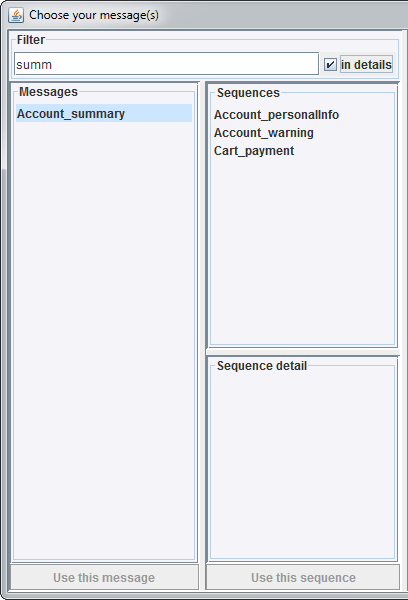
\includegraphics[scale=.5]{../screenshots/11_Filter_a.png}
  		\label{fig:filtered}
  	}\hspace{3em}%
  	\subfigure[Only in sequences names]{
  		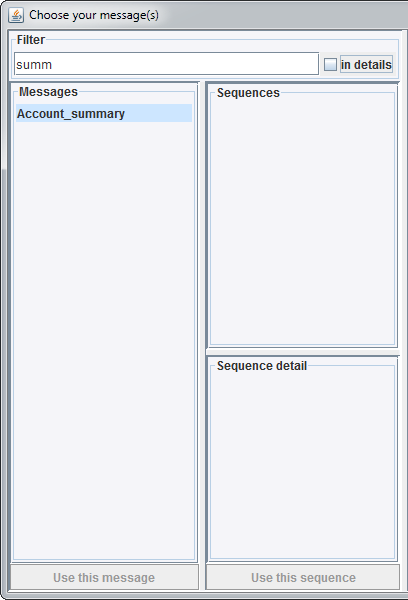
\includegraphics[scale=.5]{../screenshots/11_Filter_b.png}
  		\label{fig:filteredNotInside}
  	}
  	\caption{Filter messages and sequences}
\end{fullfigure}

\pagebreak
\subsection{Create new messages and sequences}
\label{sec:new}

\singlescreenshot{../screenshots/21_New_Partial.png}{Create new: message or sequence?}{fig:new}

A single button opens a popup bar to choose the type of the action to create.
\marginlabel{Snippets} The editor is filled with the corresponding snippet:

\begin{screenBox}[sidebyside, sidebyside align=top, 
	colbacktitle=white, coltitle=black,
	title=New message \hspace{.3\linewidth} New sequence]
\footnotesize
\begin{verbatimtab}[3]
{
	"InputElements": [{
		"Text": "",
		"Id": "",
		"Type": ""
	}],
	"OutputElements": [{
		"Text": "",
		"Id": "",
		"Type": ""
	}],
	"Id": "",
	"Language": "ita",
	"Type": "",
	"Number":  151
}
\end{verbatimtab}
\tcblower%---------------------------
\footnotesize
\begin{verbatimtab}[3]
{
	"Sequence": [
	{
		"Type": "message",
		"Value": ""
	},
	{
		"Type": "wait",
		"Value": "2000"
	}]
}
\end{verbatimtab}
\end{screenBox}

%\pagebreak
\subsection{Save messages and sequences}
\label{sec:save}

The save button reacts depending on the context.
A first element it considers is of course the type of the action. 
Then it takes into account if the action was created new or is a modification of an existing action (of which it inherits the type -- message or sequence).

\marginlabel{Save a new action}
If it was created from scratch using \newButton, the save button pops-up a bar just asking for a name.
The only way to make sure one is saving a message or a sequence is checking that the use button contains the words ``custom message'' or ``custom sequence'' (see \autoref{fig:SaveAs_FromNew}).

\begin{screenshots}
	\screenshot{../screenshots/34_SaveAs_FromNewMessage_Partial.png}{Save a new message}{fig:SaveAs_FromNewMessage}%
	\smallskip
	\screenshot{../screenshots/35_SaveAs_FromNewSequence_Partial.png}{Save a new sequences}{fig:SaveAs_FromNewSequence}%
	\caption{Save action created from scratch}
	\label{fig:SaveAs_FromNew}
\end{screenshots}

\marginlabel{Modify an existing action}
If the action is a modification of an existing action, then the save button open a more complete popup bar offering \emph{two possibilities}:
\begin{itemize}
	\item Overwrite the original action
	\item Save it as a new action (of same type)
\end{itemize}

\singlescreenshot{../screenshots/31_SaveOrSaveAs_Partial.png}{Save a modified message: overwrite or new?}{fig:saveOrSaveAs}

\marginlabel{Save as...}
If an action was not even modified, it is possible to save a copy with a new name.

\singlescreenshot{../screenshots/32_NewCopy_Partial.png}{Save an unmodified message: make a copy?}{fig:newCopy}

In any case, it is not possible to save an action with the same name as an already existing action of same type. 
Uniquness of names are case-insensitive\footnote{This is as much a technical limit than a choice to avoid confusion. Technically, actions are saved in separate files \texttt{name.json}, and Windows is case-insensitive.}.

\singlescreenshot{../screenshots/33_SaveAs_Error_Partial.png}{Given name already exists}{fig:saveAsError}

\pagebreak
\attention No correctness check is made on the grammar of the action: one can save a sequence in a message and vice-versa.
Only the Json correctness is checked before saving.

\singlescreenshot[scale=0.95]{../screenshots/36_Save_JsonError_Partial}{Json is malformed}{fig:saveAsJsonError}

%\pagebreak
\subsection{Delete messages and sequences}
\label{sec:delete}

Deleting is quite straightforward with a simple popup asking for confirmation:

\singlescreenshot{../screenshots/41_Delete_Partial.png}{Delete a message or sequence}{fig:delete}


\section{Known Issues}
\label{sec:issues}

\marginlabel{\button{Save}}
When a \msg is selected and \newButton is pressed for the creation of a new \msg, the selected \msg is not unselected.
Then, when \saveButton is pressed, it gives the previously selected message as a possible overwrite.

Similar behavior occurs if a \sequence is selected and a new \sequence is created.

\section{Possible developments}

\marginlabel{! Refresh}
Folders are scanned at startup, so a new action or deletion made outside the application is not reflected in the lists
(for instance if one updates from a version control system).
At least some kind of notification should be used.
Popup message? (easy); Autorefresh? (needs some more work).
On the other hand, the content are read on each selection. So if a message is being edited, but modified externally, the change is not reflected

\marginlabel{Functions}
For now, \socketsender allows only messages and pauses in sequences. 
If needed, it should be rather simple to add calls to Java functions defined in the code of \socketsender as part of sequences. 
This is the reason behind the sequence grammar: to be able to add a type ``function''.

Functions could have their own list, in which case the editor could show a description of what it does.
Or have a popup somewhere with a non-editable, non selectable list of possible functions.

\marginlabel{Configuration}
It could be possible to define several sources for each action type, with a priority order.
This way, one could maintain a set of messages shared between several customers, and others unique to a given customer.
In a list of 2 sources, for instance 

\begin{screenBox}
\verbatimfont{\footnotesize}%
\begin{verbatim}
"MessagesPath": {
    "actions\\GroupMessages", "actions\\CustomerMessages" }
\end{verbatim}
\verbatimfont{\normal}%
\end{screenBox}

if a message exists in both sources, the second one, \emph{more specialized} is considered.

It would be interesting to be able to block the possibility to modify, delete or create new messages in some of the sources.
This way one can make sure not to modify the \emph{parent} actions, but only the \emph{leaf versions}.
In order to avoid changing the flow too much and avoid confusion by asking each time where to save, an easy step to implement the behavior above is to consider all saves and modifications to be made in the last source of the list.

\marginlabel{Open usefull folders}
It could be handy to easily open folders defined in the configuration, for instance to update messages using TortoiseSVN.

\marginlabel{Sequence editor}
The editor is now completely text-controlled.
We could add click or drag actions, or some kind of way that would add messages into the editor when a sequence is edited.

In this case, if ever functions are also used, a similar action (and therefore list) should exists for them.

\marginlabel{Correctness check}
Could come in handy to check if the editor is writing a message or a sequence depending on a Json grammar definition.
This way, it makes it harder to mistakenly save one in another.


\end{document}